\documentclass[12pt]{article}
\usepackage{fullpage,amsmath,amssymb,graphicx}

\usepackage{setspace}
\spacing{1}

\usepackage{textpos}
\usepackage{tikz}
\usepackage{pgf}
\usepackage{amssymb}
\usepackage{enumerate}
\usepackage{xcolor}
\usepackage{graphicx}
\usepackage{subcaption}
\usepackage{tabularx}
\usepackage{colortbl}
\usepackage{multicol}
\usepackage{longtable}
\usepackage{hyperref}


\definecolor{encabezado}{rgb}{0.74, 0.83, 0.9}

\begin{document}

\hfill\\
\rule{\textwidth}{1.5pt}

\begin{minipage}[t]{85mm}
  \begin{tabular}{l}
    \textbf{\large Instituto Tecnológico de Costa Rica} \\  
    \textbf{Escuela de Ingeniería Electrónica} \\
    \textbf{Trabajo Final de Graduación} \\
    \textbf{Proyecto:} Método basado en aprendizaje reforzado \\para el control automático de una planta no lineal. \\
    \textbf{Estudiante:} Oscar Andrés Rojas Fonseca \hspace{3cm}\rule{4.5cm}{1.5pt}\\
    I Semestre 2024 \hspace{8.5cm}\textbf{Firma del asesor}
  \end{tabular}
\end{minipage}
\hfill\\
\rule{\textwidth}{1.5pt}


\section*{Bitácora de trabajo}

%\begin{table}[h]
\begin{minipage}[h]{\textwidth}
	\centering
	\begin{tabularx}{\textwidth}{|p{2cm}|X|X|p{2cm}|} 
		\hline
		\rowcolor{encabezado}
		\textbf{Fecha} & 
		\textbf{Actividad} & 
		\textbf{Anotaciones} & 
		\textbf{Horas dedicadas} \\ \hline
		% ***************************************************************
		20/02/2024 & 
	 	$\mathbf{2}.$ Estudio del funcionamiento de RLtools (C++) junto con Python. &
	 	$a)$ Revisión de opciones disponibles para el manejo de sistemas en ambos lenguajes de programación. \newline $b)$ Dadas las características, se prefiere el \textit{C++ wrapper}. \newline & 
	 	5 horas \\
	 	% ***************************************************************
	 	21/02/2024 & 
	 	$\mathbf{3}.$ Estudio de la comunicación entre el sistema (planta) y el módulo de control al sistema (Red neuronal). & 
	 	$a)$ Revisión de la teoría correspondiente en \cite{DataScience}. \newline 
	 	$b)$ Revisión de ejemplos de funcionamiento del MPC \cite{Airdaldi2023}. \newline & 
	 	5 horas \\	
	 	% ***************************************************************
	 	22/02/2024 & 
	 	$\mathbf{4}.$ Pruebas realizadas con la librería RLtools. & 
	 	$a)$ Instalación de dependencias y pruebas de paquetería \cite{rltools}. \newline  & 
	 	6 horas \\
	 	% ***************************************************************
	 	23/02/2024 & 
	 	$\mathbf{5}.$ Prueba de entrenamiento con datos reales del PAMH. & 
	 	$a)$ Se ejecutó el script $RNAM\_Real.py$ con una primera versión de los datos recolectados. Sin exito por tiempo de ejecución muy largo. \newline & 
	 	5 horas \\
	 	% ***************************************************************
	 	\hline
		\multicolumn{3}{|r|}{Total de horas de trabajo:} & 21 horas \\ 
	 	\hline                 
	\end{tabularx}
\end{minipage}
%\end{table}


% *****************************************************************************
% *****************************************************************************
% *****************************************************************************
\newpage

\section*{Contenidos de actividades}

\subsection*{C++ Wrapper}

Para la utilización de algoritmos definidos en $C++$ como es el caso de la libretía RLtools y aplicarlos a modelos o bases en $Python$, es necesaria la "traduccción" o adaptación para manejar los dos sistemas, donde es posible traducir todo el modelo previo a $C++$ o la implementación de un \textit{C++ wrapper}, en este caso preferido para no afectar el modelo de entrenamiento de la red neuronal mimetizadora, anteriormente definida, y su control en tiempo continuo.

\subsection*{Control predictivo del modelo (MCU)}

La estructura de comunicación entre el sistema y el modelo de control mediante maching learning se efectua con base en funciones de optimización, donde se generan acciones controladas en cada paso para controlar alguna característica ($\mathbf{\hat{F}}$) y se toma la primera muestra de dicha acción ($\hat{x}_{k+1}$) para variar la respuesta del controlador enviada al sistema ($\mathbf{u}_j$), esto independiente y apllicable a sistemas lineales o no lineales. El proceso se simplifica en la Fig. \ref{fig:mpc}.


\begin{figure}[h]
	\centering
	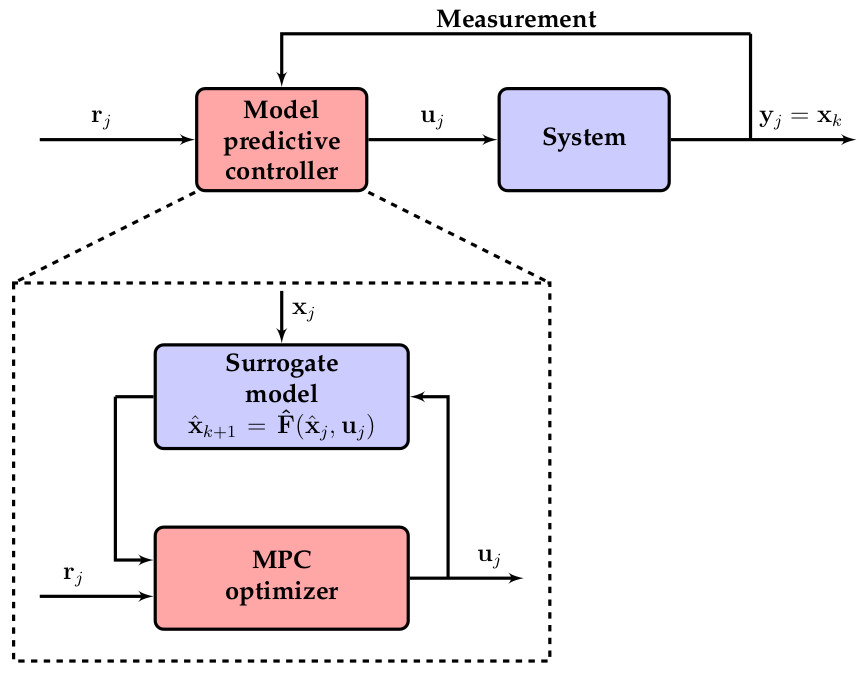
\includegraphics[scale=0.35]{Fig/MPC.png}
	\caption{Esquemático del control predictivo del modelo (MPC) \cite{DataScience}.}
	\label{fig:mpc}
\end{figure}


\subsection*{Pruebas de funcionamiento}

Luego de instalar las dependencias necesarias para un primer entrenamiento usando \textit{RLtools}, se logró el entrenamiento del modelo más simple de la librería, el péndulo con TD3. Ejemplo de esto se muestra en la Fig. \ref{fig:pendtraining}.


\begin{figure}[h]
	\centering
	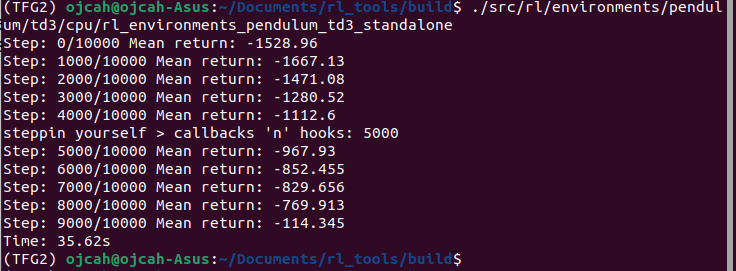
\includegraphics[scale=0.5]{Fig/PruebaPendulo.png}
	\caption{Entrenamiento preliminar del péndulo con RLtools.}
	\label{fig:pendtraining}
\end{figure}






\newpage

\section*{Referencias}
\renewcommand\refname{}
\bibliographystyle{IEEEtran}
\bibliography{references}





\end{document}